% !TEX program = xelatex
\documentclass[12pt]{beamer}

% Tema y configuración básica
\usetheme{metropolis}
\setbeamertemplate{frame numbering}[fraction]
\setbeamercolor{background canvas}{bg=white}

% Logo en todas las diapositivas
\logo{
\includegraphics[height=1cm]{images/logo_uct.png}}

% Información institucional
\institute{Universidad Católica de Temuco\\
          Facultad de Ingeniería}

\author{%
    \textbf{Integrantes:}\\[0.3cm]
    Joaqu\'{i}n Carrasco\\[0.3cm]
    Benjamin Cabrera\\[0.3cm]
    Leonardo Ch\'{a}vez\\[0.3cm]
    \textbf{Profesor:} Guido Mellado\\[0.3cm]
    \textbf{Asignatura:} Programaci\'{o}n II\\[0.3cm]
    \textbf{Secci\'{o}n:} 2%
}

% Paquetes básicos
\usepackage[spanish]{babel}
\usepackage[utf8]{inputenc}
\usepackage[T1]{fontenc}
\usepackage{graphicx}
\usepackage{tikz}
\usepackage{listings}
\usepackage{xcolor}

% Configuración de listados de código
\lstset{
    basicstyle=\ttfamily\small,
    breaklines=true,
    captionpos=b,
    commentstyle=\color{gray},
    frame=single,
    numbers=left,
    numberstyle=\tiny\color{gray},
    keywordstyle=\color{blue},
    showstringspaces=false,
    stringstyle=\color{orange},
    tabsize=2
}

% Configuración de hipervínculos (al final para evitar conflictos)
\usepackage{bookmark}
\usepackage{hyperref}
\hypersetup{
    pdfencoding=auto,
    unicode=true,
    colorlinks=true,
    linkcolor=blue,
    filecolor=magenta,
    urlcolor=cyan,
    pdftitle={Sistema de Gestión de Restaurante},
    pdfauthor={Joaquín Carrasco Durán},
    pdfsubject={Presentación Evaluación 2},
    pdfkeywords={restaurante, python, programación}
}

% Información del título
\title{Sistema de Gestión de Restaurante}
\subtitle{Evaluación N°2 --- Programación II}
\date{\today}
% La información de autores e institución ya está definida arriba
% \author y \institute se mantienen como se definieron al inicio del documento

\begin{document}

% Título
\begin{frame}[plain]
    \titlepage{}
\end{frame}

% Contenido
\begin{frame}{Contenidos}
    \tableofcontents
\end{frame}

\section{Introducción}
\begin{frame}{Descripción del Sistema}
    \begin{itemize}
        \item Sistema de gestión para restaurante implementado en Python
        \item Manejo de inventario, pedidos y generación de boletas
        \item Interfaz gráfica intuitiva con CustomTkinter
        \item Implementación de patrones de diseño para una arquitectura robusta
    \end{itemize}
\end{frame}

\section{Arquitectura}
\begin{frame}{Patrones de Diseño - Visión General}
    \begin{itemize}
        \item Se implementaron cuatro patrones de diseño principales
        \item Cada patrón resuelve un problema específico
        \item Los patrones trabajan en conjunto para crear una arquitectura robusta
        \item Facilitan el mantenimiento y la extensibilidad del sistema
    \end{itemize}
\end{frame}

\begin{frame}{Patrón Facade}
    \begin{exampleblock}{¿Qué es Facade?}
        \begin{itemize}
            \item Patrón estructural que proporciona una interfaz simplificada
            \item Oculta la complejidad del sistema
            \item Reduce el acoplamiento entre componentes
        \end{itemize}
    \end{exampleblock}
    \begin{alertblock}{Implementación en el Proyecto}
        \begin{itemize}
            \item Clase \texttt{BoletaFacade}:
            \begin{itemize}
                \item Simplifica la generación de boletas
                \item Maneja la creación de PDFs
                \item Coordina la visualización de documentos
            \end{itemize}
        \end{itemize}
    \end{alertblock}
\end{frame}

\begin{frame}{Patrón Observer}
    \begin{exampleblock}{¿Qué es Observer?}
        \begin{itemize}
            \item Patrón de comportamiento
            \item Define una dependencia uno-a-muchos
            \item Notifica automáticamente cambios a los observadores
        \end{itemize}
    \end{exampleblock}
    \begin{alertblock}{Implementación en el Proyecto}
        \begin{itemize}
            \item Actualización de la interfaz gráfica:
            \begin{itemize}
                \item Refleja cambios en tiempo real
                \item Mantiene sincronizado el estado
                \item Separa la lógica de negocio de la presentación
            \end{itemize}
        \end{itemize}
    \end{alertblock}
\end{frame}

\begin{frame}{Patrón Singleton}
    \begin{exampleblock}{¿Qué es Singleton?}
        \begin{itemize}
            \item Patrón creacional
            \item Garantiza una única instancia
            \item Proporciona un punto de acceso global
        \end{itemize}
    \end{exampleblock}
    \begin{alertblock}{Implementación en el Proyecto}
        \begin{itemize}
            \item Clase \texttt{Stock}:
            \begin{itemize}
                \item Control centralizado del inventario
                \item Evita inconsistencias en el estado
                \item Gestión thread-safe de recursos
            \end{itemize}
        \end{itemize}
    \end{alertblock}
\end{frame}

\begin{frame}{Patrón Factory}
    \begin{exampleblock}{¿Qué es Factory?}
        \begin{itemize}
            \item Patrón creacional
            \item Delega la creación de objetos
            \item Permite extensibilidad y flexibilidad
        \end{itemize}
    \end{exampleblock}
    \begin{alertblock}{Implementación en el Proyecto}
        \begin{itemize}
            \item Clase \texttt{Menu\_catalog}:
            \begin{itemize}
                \item Crea elementos del menú dinámicamente
                \item Facilita la adición de nuevos productos
                \item Mantiene consistencia en la creación
            \end{itemize}
        \end{itemize}
    \end{alertblock}
\end{frame}

\begin{frame}{Interacción entre Patrones}
    \begin{itemize}
        \item \textbf{Facade + Observer}
        \begin{itemize}
            \item Notificación de cambios en documentos
            \item Actualización automática de vistas
        \end{itemize}
        \item \textbf{Singleton + Factory}
        \begin{itemize}
            \item Validación centralizada de recursos
            \item Creación controlada de productos
        \end{itemize}
        \item \textbf{Observer + Singleton}
        \begin{itemize}
            \item Monitoreo del estado del inventario
            \item Actualización en tiempo real del UI
        \end{itemize}
    \end{itemize}
\end{frame}

\section{Implementación}
\begin{frame}{Estructura del Proyecto}
    \begin{itemize}
        \item \textbf{Módulos Principales}
        \begin{itemize}
            \item \texttt{Restaurante.py}: Punto de entrada y GUI principal
            \item \texttt{Stock.py}: Gestión de inventario (Singleton)
            \item \texttt{Menu\_catalog.py}: Catálogo de productos (Factory)
            \item \texttt{BoletaFacade.py}: Generación de documentos (Facade)
        \end{itemize}
        \item \textbf{Clases de Soporte}
        \begin{itemize}
            \item \texttt{ElementoMenu.py}: Productos del menú
            \item \texttt{Ingrediente.py}: Componentes base
            \item \texttt{Pedido.py}: Gestión de órdenes
        \end{itemize}
    \end{itemize}
\end{frame}

\section{Funcionalidades}
\begin{frame}{Diagrama de Clases}
    \centering
    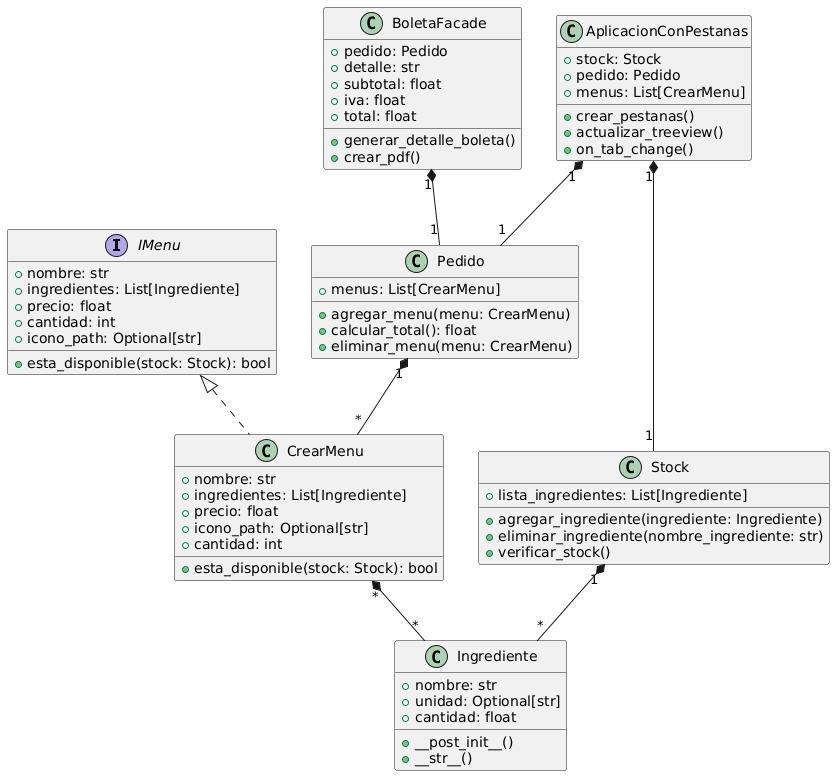
\includegraphics[height=0.8\textheight]{images/diagrama.png}
\end{frame}

\begin{frame}{Explicación del Diagrama de Clases}
    \centering
    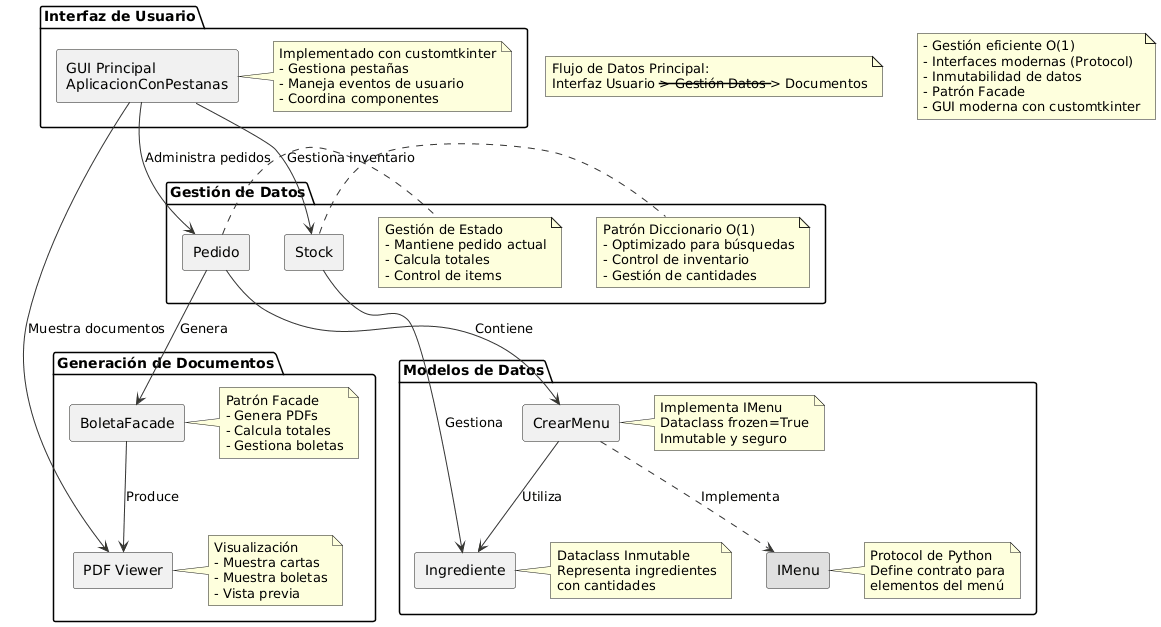
\includegraphics[width=0.95\textwidth,height=0.8\textheight,keepaspectratio]{images/explicacion_diagrama.png}
\end{frame}

\section{Implementación}
\begin{frame}[fragile]{Carga de Ingredientes}
    \begin{itemize}
        \item \textbf{Botón ``Cargar CSV''}:
        \begin{itemize}
            \item Abre selector de archivo
            \item Valida formato CSV
            \item Actualiza inventario
        \end{itemize}
    \end{itemize}
    \begin{exampleblock}{Código}
        \begin{verbatim}
def cargar_csv(self):
    archivo = filedialog.askopenfilename(
        filetypes=[("CSV files", "*.csv")])
    if archivo:
        self.df_csv = pd.read_csv(archivo)
        self.actualizar_stock()
        \end{verbatim}
    \end{exampleblock}
\end{frame}

\begin{frame}[fragile]{Gestión de Stock}
    \begin{itemize}
        \item \textbf{Control de Inventario}:
        \begin{itemize}
            \item Verificación automática
            \item Reserva de ingredientes
            \item Patrón Singleton
        \end{itemize}
    \end{itemize}
    \begin{exampleblock}{Validación de Stock}
        \begin{verbatim}
def verificar_stock(self, nombre, cantidad):
    ingrediente = self.ingredientes.get(nombre)
    return ingrediente and ingrediente.cantidad >= cantidad
        \end{verbatim}
    \end{exampleblock}
\end{frame}

\begin{frame}[fragile]{Procesamiento de Pedidos}
    \begin{itemize}
        \item \textbf{Botón ``Agregar al Pedido''}:
        \begin{itemize}
            \item Verifica disponibilidad
            \item Reserva ingredientes
            \item Actualiza interfaz
        \end{itemize}
    \end{itemize}
    \begin{exampleblock}{Gestión de Pedido}
        \begin{verbatim}
def agregar_al_pedido(self, menu_item):
    if self.stock.reservar_ingredientes(menu_item):
        self.pedido.agregar_item(menu_item)
        self.actualizar_vista()
        \end{verbatim}
    \end{exampleblock}
\end{frame}

\begin{frame}[fragile]{Generación de Boleta}
    \begin{itemize}
        \item \textbf{Botón ``Generar Boleta''}:
        \begin{itemize}
            \item Crea PDF con detalles
            \item Usa patrón Facade
            \item Muestra vista previa
        \end{itemize}
    \end{itemize}
    \begin{exampleblock}{BoletaFacade}
        \begin{verbatim}
def generar_boleta(self):
    facade = BoletaFacade(self.pedido)
    facade.generar_boleta()
    facade.mostrar_boleta()
        \end{verbatim}
    \end{exampleblock}
\end{frame}

\begin{frame}[fragile]{Visualización de PDFs}
    \begin{itemize}
        \item \textbf{Botón ``Mostrar PDF''}:
        \begin{itemize}
            \item Vista previa del documento
            \item Navegación entre páginas
            \item Zoom y controles interactivos
        \end{itemize}
    \end{itemize}
    \begin{exampleblock}{Visor PDF Personalizado}
        \begin{verbatim}
def mostrar_pdf(self, archivo):
    visor = PDFViewer(self.ventana)
    visor.load_pdf(archivo)
    visor.mostrar()
        \end{verbatim}
    \end{exampleblock}
\end{frame}

\begin{frame}[fragile]{Gestión del Menú}
    \begin{itemize}
        \item \textbf{Botón ``Eliminar del Menú''}:
        \begin{itemize}
            \item Remueve elementos seleccionados
            \item Actualiza catálogo en tiempo real
            \item Libera ingredientes reservados
        \end{itemize}
    \end{itemize}
    \begin{exampleblock}{Eliminación de Elementos}
        \begin{verbatim}
def eliminar_del_menu(self, item_id):
    if item_id in self.pedido.items:
        self.stock.liberar_ingredientes(item_id)
        self.pedido.eliminar_item(item_id)
        self.actualizar_vista()
        \end{verbatim}
    \end{exampleblock}
\end{frame}

\begin{frame}[fragile]{Gestión del Menú - Continuación}
    \begin{itemize}
        \item \textbf{Botón ``Limpiar Pedido''}:
        \begin{itemize}
            \item Reinicia el pedido actual
            \item Libera todos los ingredientes
            \item Actualiza la interfaz
        \end{itemize}
    \end{itemize}
    \begin{exampleblock}{Reinicio de Pedido}
        \begin{verbatim}
def limpiar_pedido(self):
    for item in self.pedido.items:
        self.stock.liberar_ingredientes(item)
    self.pedido.limpiar()
    self.actualizar_total()
        \end{verbatim}
    \end{exampleblock}
\end{frame}

\begin{frame}{Conclusiones}
    \begin{itemize}
        \item \textbf{Aprendizajes Clave}:
        \begin{itemize}
            \item Aplicación práctica de patrones de diseño
            \item Importancia del desacoplamiento de componentes
            \item Manejo efectivo de eventos y estados
        \end{itemize}
        \vspace{0.5cm}
        \item \textbf{Desafíos Superados}:
        \begin{itemize}
            \item Sincronización de GUI con lógica de negocio
            \item Manejo consistente del estado global
            \item Validación robusta de datos
        \end{itemize}
    \end{itemize}
\end{frame}

\end{document}